\documentclass{article}
\usepackage[utf8]{inputenc}
\usepackage{graphicx}
\usepackage{amsfonts}       % blackboard math symbols

\setlength{\parindent}{1cm} % espaçamento do parágrafo
\usepackage{geometry} % configurar layout da página
\usepackage{setspace} % configurar o espaçamento de linhas
\usepackage{indentfirst} % alinhamento do texto, parágrafos

\graphicspath{ {./images/} }

\usepackage{float} % tabela que nao fica fixa

\usepackage{siunitx}  % Package perfeita pra notacao cientifica
\RequirePackage{amsmath,amsthm,amssymb,hyperref} % Math 

\title{ENGC46 - Síntese de Circuitos: Trabalho II}
\date{Semestre Letivo Suplementar 2020 - Universidade Federal da Bahia}
\author{Henrique Nunes Poleselo}

\begin{document}

\maketitle

\section{Especificações}
O objetivo é projetar um filtro passa-baixas utilizando redes passivas e depois converte-lo em rede ativa utilizando a transformação de Bruton de forma a eliminar os indutores da rede passiva. Especificações do projeto:
\begin{itemize} 
    \item Banda passante: 1Hz - 28kHz
    \item Banda de rejeição: 28kHz - 123.3kHz
    \item Amax: 0.1dB
    \item Amin: 40dB
    \item Impedância de carga e da fonte: 1k
    \item Função de aproximação: Butterworth
    \item Técnica de Bruton
\end{itemize}


\section{Projeto}
A partir dos requisitos do projeto, utilizando-se a expressão para a determinação de ordem mínima do filtro:
\begin{equation}
     \epsilon = \sqrt{10^{A_m_a_x/10}-1} = 0.1526.
\end{equation}

\begin{equation}
     n > \frac{log(\frac{10^{A_m_i_n/10}-1}{10^{A_m_i_n/10}-1})}{log(\frac{\omega p}{\omega s})^2} = 4.37 \therefore n = 5.
\end{equation}

Como a ordem é ímpar, a rede possui a seguinte arquitetura:

\begin{center}
\centering
  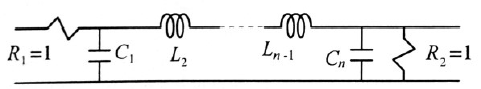
\includegraphics[scale=0.8]{img/arquiteturaDaRede.png}
\end{center}

No projeto em questão as resistências R1 e R2 são consequentemente 1k\si{\ohm}. Além disso sabe-se que a ordem mínima é 5, portanto a arquitetura do filtro em questão terá 3 capacitores e 2 indutores. Para o dimensionamento dos componentes do circuito acima, utilizou-se as expressões que fornecem diretamente o valor (normalizado) dos componentes para a aproximação de Butterworth:

\begin{equation}
    C_k = 2 \cdot \epsilon^{1/n} \cdot sen(\frac{(2k-1)\pi}{2n}).
\end{equation}

Sendo a expressão pros capacitores, para k ímpar.

\begin{equation}
    L_k = 2 \cdot \epsilon^{1/n} \cdot sen(\frac{(2k-1)\pi}{2n}).
\end{equation}

Para os indutores, que no caso são os termos pares.

Os cálculos foram manuais, portanto em anexo a este relatório é possível vizualiza-los, apesar dos mesmos estarem relativamente bagunçados e informais. Na tabela 1 encontram-se os valores normalizados dos componentes.

\begin{table}[H]
\centering
\begin{tabular}{|c|c|c|}
\hline
Componente & Normalizado \\ \hline
C1 & \num{0.4243}F  \\ \hline
C3 & \num{1.3732}F  \\ \hline
C5 & \num{0.4243}F  \\ \hline
L2 & \num{1.1109}H  \\ \hline
L4 & \num{1.1109}H  \\ \hline
\end{tabular}
\caption{Valores normalizados.}
\end{table}

Para a verificação comportamental do filtro através de simulação, fez-se a desnormalização dos valores encontrados, tal desnormalização foi feita utilizando as relações que dependem da frequência de corte \textit{fp} e da impedância:

\begin{equation}
    Ck_d_e_s = \frac{C_k}{a \cdot b}.
\end{equation}

E para a desnormalização do indutor:
\begin{equation}
    Lk_d_e_s = \frac{L_k \cdot b}{a}.
\end{equation}

No projeto em questão, os valores da desnormalização da frequência e da impedância \textit{a} e \textit{b} são, respectivamente: \num{2\pi28e3} e \num{1e3}.

\begin{table}[H]
\centering
\begin{tabular}{|c|c|c|}
\hline
Componente & Normalizado  & Desnormalizado  \\ \hline
C1 & \num{0.4243}F & \num{2.41e-9}F \\ \hline
C3 & \num{1.3732}F & \num{7.805e-9}F \\ \hline
C5 & \num{0.4243}F & \num{2.41e-9}F \\ \hline
L2 & \num{1.1109}H & \num{6.314e-3}H \\ \hline
L4 & \num{1.1109}H & \num{6.314e-3}H \\ \hline
\end{tabular}
\caption{Comparativo entre os componentes normalizados e desnormalizados de acordo com a frequência de corte \textit{fp} de 28kHz e impedância de 1k.\si{\ohm}.}
\end{table}


A rede passiva LC montada no LTSpice com os valores desnormalizados foi:

\begin{center}
\centering
  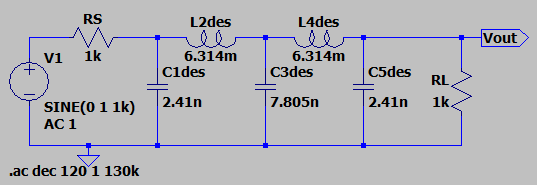
\includegraphics[scale=0.8]{img/ladder.png}
\end{center}

A nível de validação, com a simulação do circuito acima feita, avaliou-se a magnitude (em módulo) da rede simulada na frequência de corte \textit{fp} (28kHz) e a magnitude em 1Hz, ao fazer a diferença entre ambas, obteve-se:

\begin{equation}
    6.1275dB - 6.0206dB = 0.1069dB.
\end{equation}

Como uma das especificações era de 0.1dB de atenuação máxima na banda passante, mostra que o filtro teve um comportamento esperado. 

O mesmo foi feito na banda de rejeição, neste caso na frequência \textit{fp} (123.2kHz) e na frequência de corte (reiterando que as magnitudes estão em módulo):
\begin{equation}
    53.9605dB - 6.1275dB = 47.833dB.
\end{equation}

A resposta em frequência completa da rede passiva se encontra no final deste relatório juntamente com uma comparação à resposta em frequência da implementação do mesmo em filtro ativo utilizando a transformação de Bruton.

Para a implementação da rede passiva em uma rede ativa, utilizou-se a transformação de Bruton (escalonamento dos componentes do circuito por $1/s$), como especificado no projeto. Portanto os resistores se tornam capacitores, indutores se tornam resistores e capacitores se tornam supercapacitores. A rede escalonada ficou da seguinte forma: 

\begin{center}
\centering
  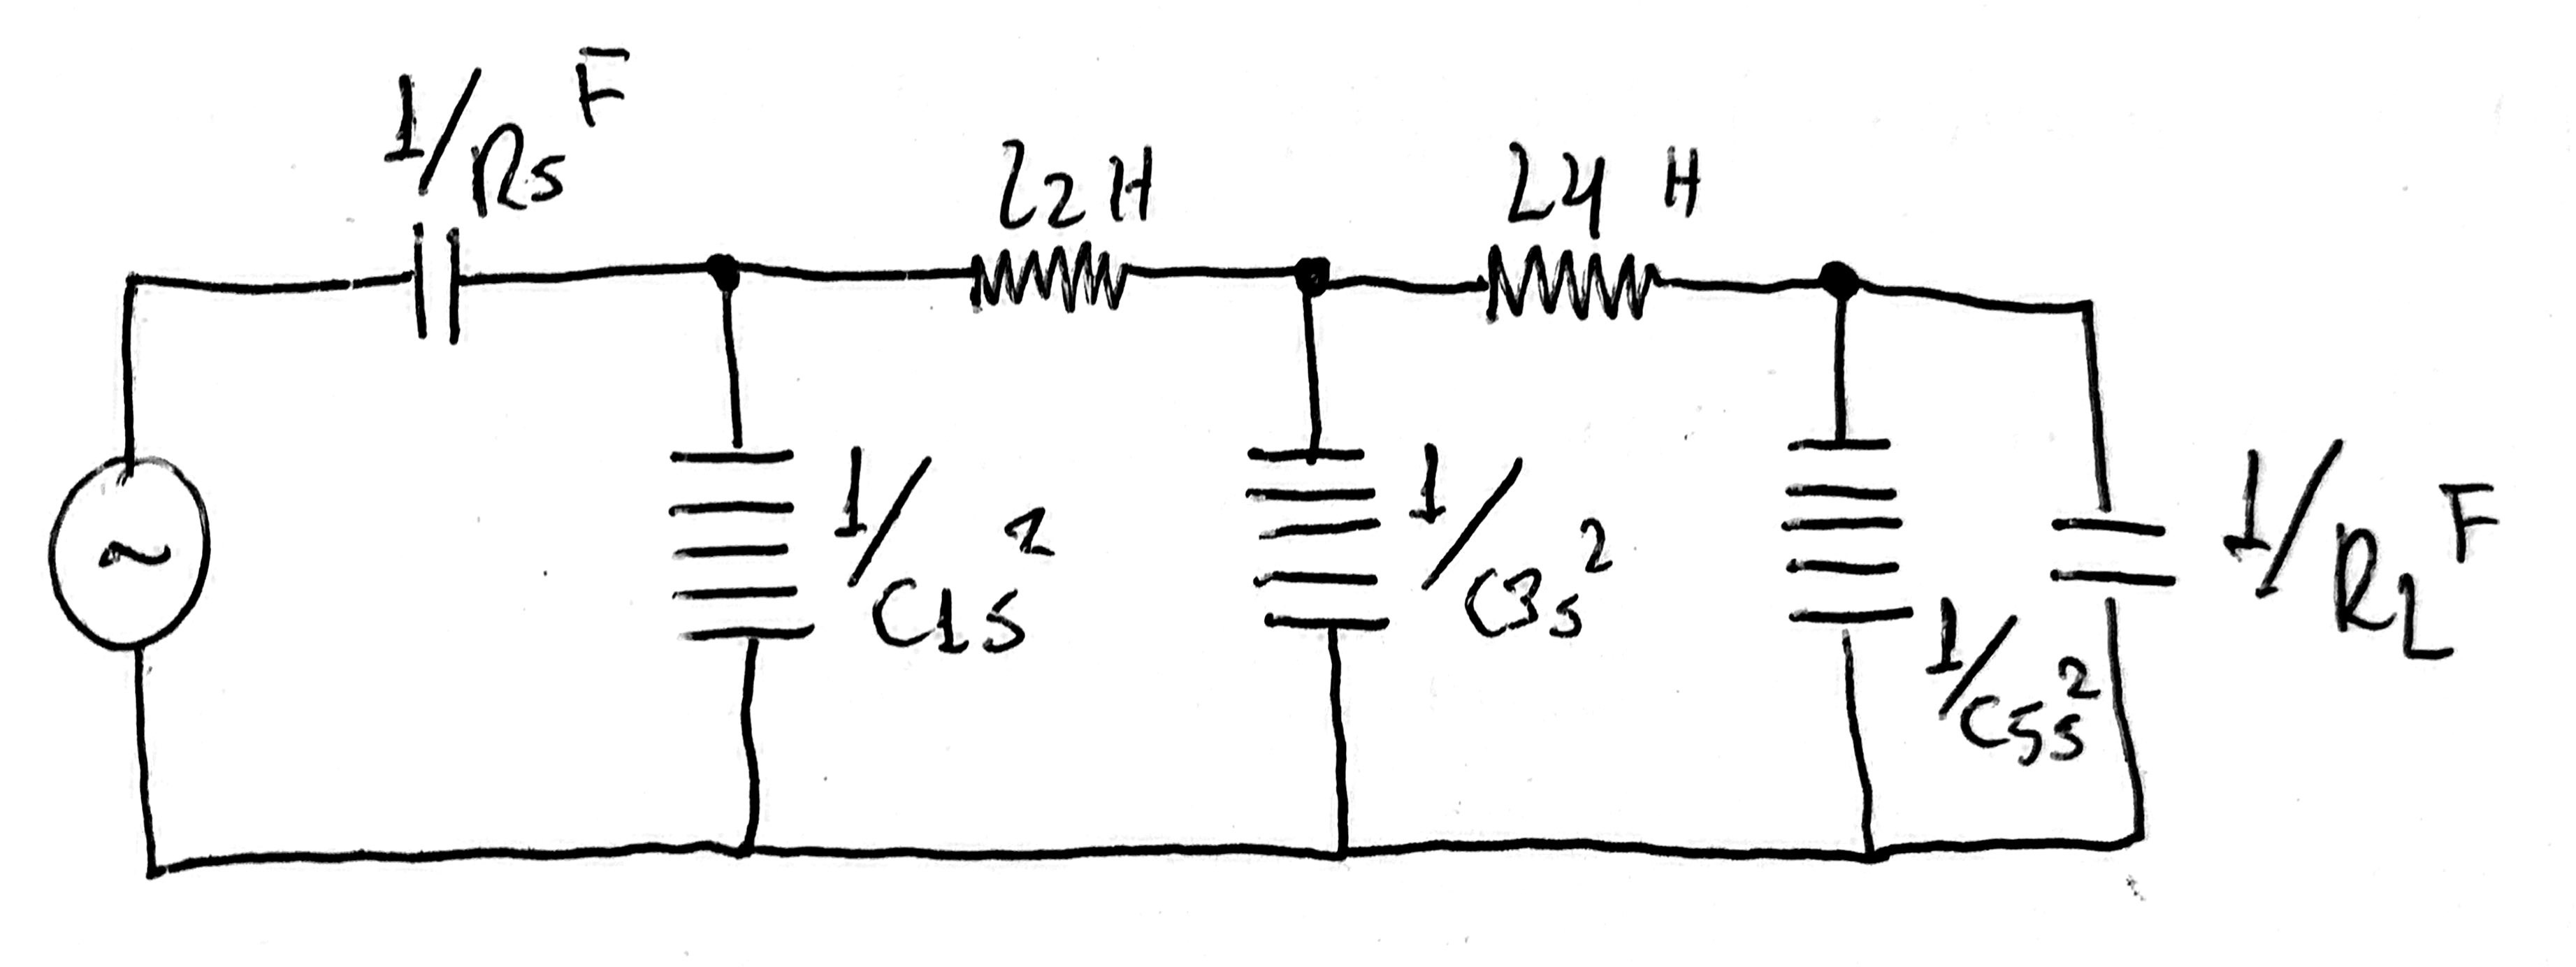
\includegraphics[scale=0.08]{img/circuitoTransf.JPG}
\end{center}

No entanto, apesar de eliminar os indutores com a transformação de Bruton, obtem-se um supercapacitor (FNDR), para a implementação do mesmo foi utilizada a implementação com \textit{GIC's}, transformando a rede passiva em uma rede ativa propriamente dita. Lembrando que o \textit{GIC} segue o seguinte formato:

\begin{center}
\centering
  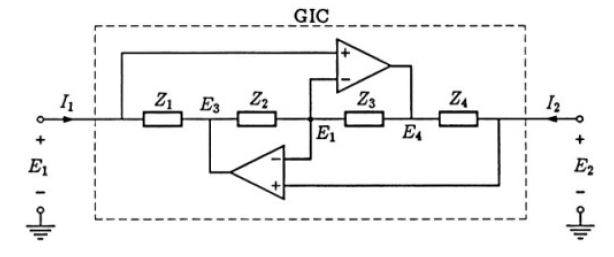
\includegraphics[scale=0.6]{img/gic.png}
\end{center}

Portanto, basta escolher os valores das impedâncias \textit{Z1}, \textit{Z2}, \textit{Z3} e \textit{Z4} e adicionar um capacitor a mais com o valor do capacitor original (C1,C3 e C5) de forma a se ter $s^2$, i.e: implementar o supercapacitor. Para as 4 impedâncias em questão, foram escolhidos 3 resistores de 1\si{\ohm} e 1 capacitor de 1F.

O circuito final com os valores projetados pode ser visto na imagem abaixo:
\begin{center}
\centering
  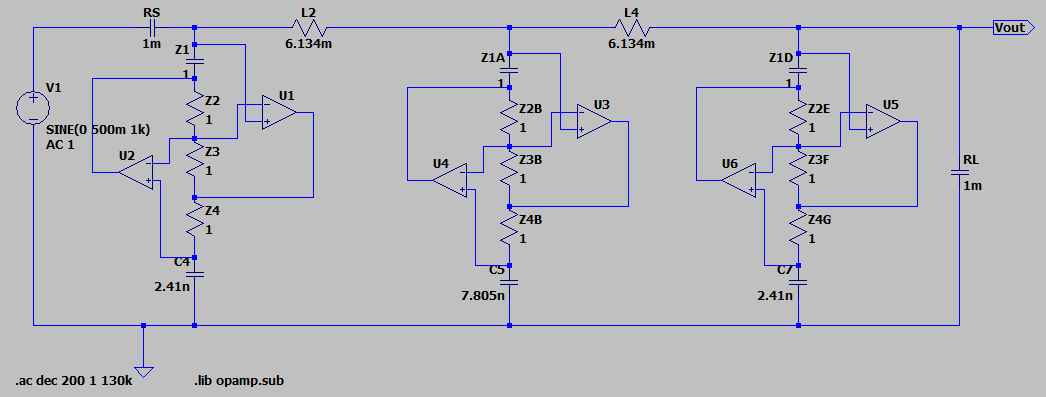
\includegraphics[scale=0.5]{img/passivoativo.png}
\end{center}

Importante notar que o valor do capacitor adicional, na figura acima (C4, C5 e C7), tiveram seus valores arbitrados como sendo o próprio valor do capacitor original desnormalizado. O mesmo procedimento de validação que foi feito na rede passiva para análise dos requisitos de projeto (magnitude em módulo na frequência de 1Hz, \textit{fp} e \textit{fs}):

\begin{equation}
    6.02117dB - 6.02106dB = 0.0001096dB.
\end{equation}

\begin{equation}
    55.59777dB - 6.0211dB = 49.5766dB.
\end{equation}

Portanto os requisitos da máxima atenuação na banda passante e mínima atenuação na banda de rejeição continuaram sendo respeitados. 


Comparação entre a rede passiva LC e a rede ativa transformada:
\begin{center}
\centering
  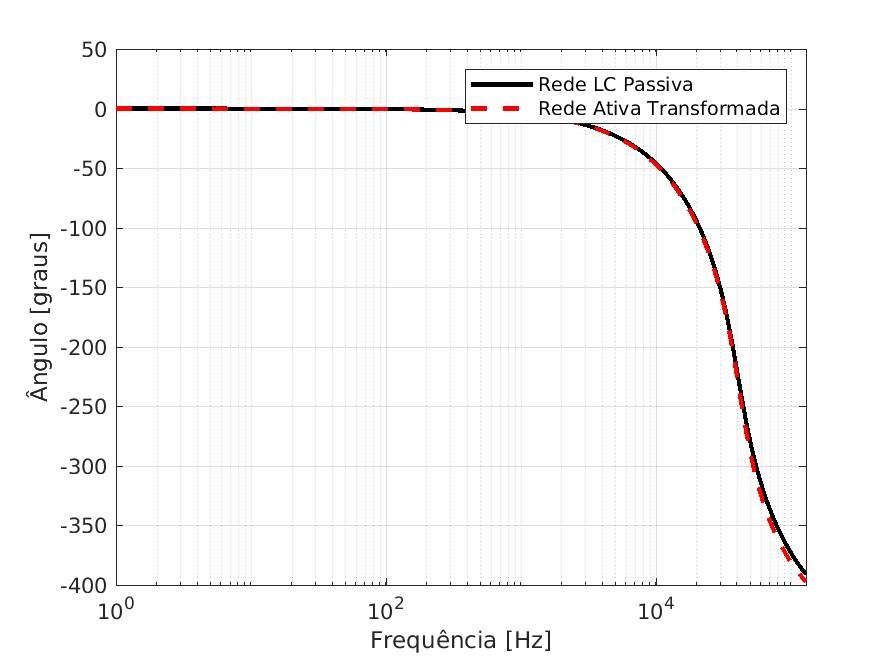
\includegraphics[scale=0.7]{img/phase.png}
\end{center}

\begin{center}
\centering
  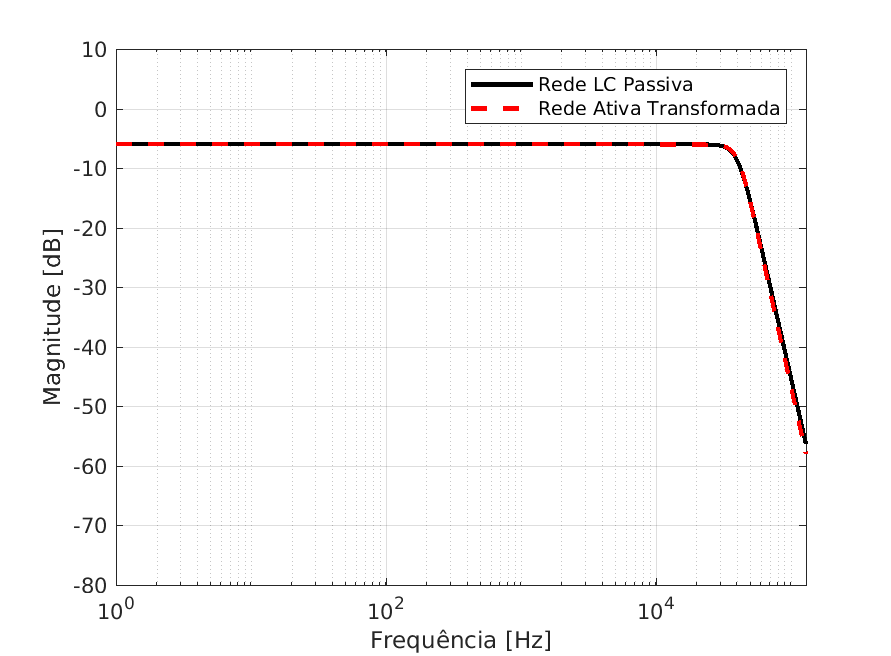
\includegraphics[scale=0.7]{img/magnitude.png}
\end{center}

Resposta em frequência da rede ativa e passiva com ampliação em torno da banda passante:

\begin{center}
\centering
  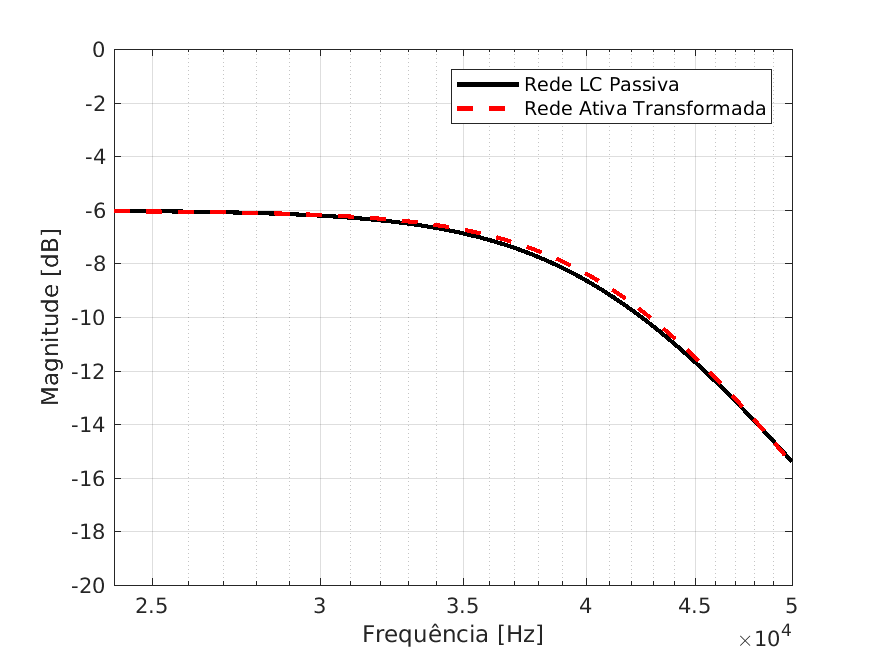
\includegraphics[scale=0.7]{img/magnitudebandpass.png}
\end{center}

Resposta em frequência da rede ativa e passiva com ampliação em torno da banda de rejeição:

\begin{center}
\centering
  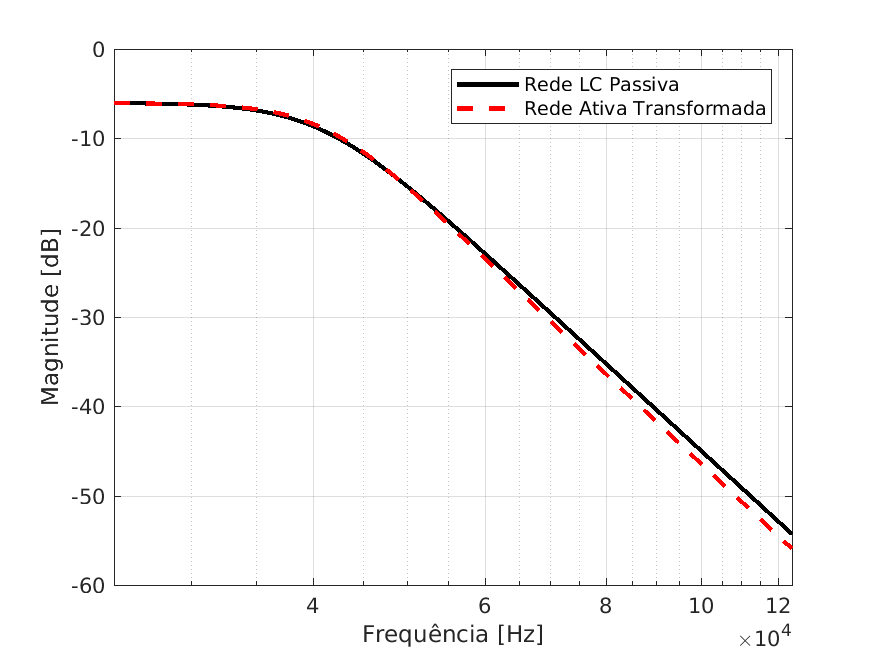
\includegraphics[scale=0.7]{img/magnitudebandstop.png}
\end{center}

Tabela comparativa das duas implementações baseado nos critérios de projeto:
\begin{center}
\centering
  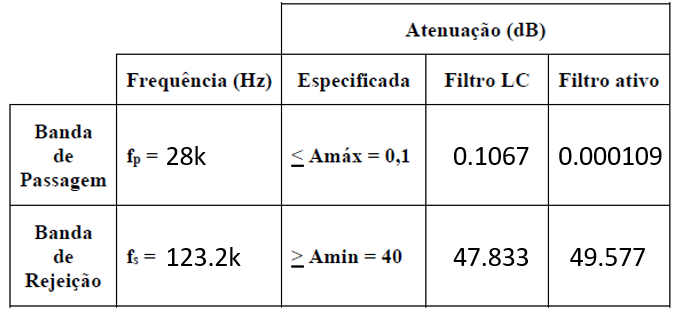
\includegraphics[scale=0.5]{img/tabelapreeenchida.png}
\end{center}

\end{document}